\documentclass[conference]{IEEEtran}
\usepackage{amsmath,amssymb,graphicx}
\usepackage{booktabs}
\usepackage{tikz}
\usetikzlibrary{positioning,arrows.meta,fit,calc}

% Built on the course template report_template.tex (IEEEtran, conference).
% Compile with: pdflatex report.tex   (run twice for references)

\newcommand{\todo}[1]{\textbf{[TODO: #1]}}

\title{Slalom Challenge: Backward DP Planning\\ with Model-Based Bounds and Path Tracking}
\author{
  \IEEEauthorblockN{[Your Name]}
  \IEEEauthorblockA{[Student ID] \\
  Learning-Based Control for Mobility Systems, 2026}
}

\begin{document}
\maketitle

% =====================================================================
\section{Problem Statement}
% =====================================================================
\textbf{Task and submission.} A PyChrono 10.0.0 BMW~E90 (TMeasy tires,
$\mu=0.9$) must pass eight cones at $X_j=20+15j$\,m, $Y_j=0$, alternately on
$+Y$ (even $j$) and $-Y$ (odd $j$), and reach $X_{\rm REF}=145$\,m as fast as
possible (repository commit \texttt{e05dace}). I solved \emph{both} modes with
the same method; the result to evaluate is \textbf{Full mode (v2):
14.985\,s} \todo{confirm the evaluated mode in the e-mail}. Easy mode
(16.333\,s) is submitted as supporting work.

\textbf{Official problem.} Minimize the finish time $t_f$ over the commands,
subject to the vehicle dynamics, command bounds, $-1\le v_x\le 12$\,m/s,
$\dot X_{\rm REF}\le 12$\,m/s, $|\psi|\le 1.3$\,rad, the $4.7\times1.9$\,m
COM-centred footprint never touching a cone or leaving the road
($|Y|\le5.5$\,m), and ordered forward gate crossings with
$\sigma_j\bigl(Y_{\rm REF}(t_j)-Y_j\bigr)>0$, $t_f\le60$\,s. The only cone
rule is \emph{clearance $>0$}; no lateral gate distance or safety margin is
prescribed.

\textbf{State and action.} Full mode: measured state
$s=(X_{\rm REF},Y_{\rm REF},\psi,v_x,v_y,r,\delta)$ every $0.02$\,s plus the
previously applied steering; action
$u=(u_s^{\rm req},a_x^{\rm req})\in[-0.8,0.8]\times[-7,7]$\,m/s$^2$, converted
by the fixed input adapter (steering slew $0.04$ per step, open-loop pedal map).
Easy mode: a list of integer moves $(m,n)$, $m\in\{1..5\}$, $n\in\{-4..4\}$,
on a $1\times0.5$\,m lattice with $\Delta=0.5$\,s stages, driven by the
professor's fixed tracker.

\textbf{My surrogate objective.} I plan the REF point on a lattice with a
discrete DP whose state is $z_k=(X_k,Y_k,p_k)$, where $p_k$ is the previous
move (state augmentation: the speed and turning bounds compare
$V_k,\chi_k$ with $V_{k-1},\chi_{k-1}$). The stage cost is $1$ (one
$\Delta=0.5$\,s stage); in Full mode the move that crosses the finish line
costs only the fraction of the stage it needs, so the DP minimizes the
\emph{planned time to the line}. Constraints become infeasible transitions
(equivalent to a failure cost $M>K_{\max}$), and the finish is absorbing. The
planned time is only a surrogate for $t_f$: a tracking controller must realize
the plan on the real plant, so every design was validated by its PyChrono finish
time and minimum footprint clearance. Table~\ref{tab:rules} separates the
official rules, the professor's suggested values and my own choices.

\begin{table}[t]
\centering
\caption{Official rules vs.\ suggested values vs.\ my design choices}
\label{tab:rules}
\footnotesize
\setlength{\tabcolsep}{3pt}
\begin{tabular}{@{}lll@{}}
\toprule
Quantity & Source & Value used \\
\midrule
Cone clearance & rule & $>0$ (no margin required)\\
Speed / heading & rule & $v_x,\dot X_{\rm REF}\le12$\,m/s, $|\psi|\le1.3$\\
Easy gate margin & mine & 2.0\,m (official: $d_j>0$)\\
Easy $|\Delta\chi|$, $V|\Delta\chi|/\Delta$ & suggested & 0.31\,rad, 6\,m/s$^2$\\
\quad relaxed to & mine & 0.5\,rad, 8\,m/s$^2$ (tested)\\
Full max speed & mine & 11.5\,m/s\\
Full acceleration & model & $\int dv/a_{\max}(v)\le\Delta$\\
Full body / road margin & mine & 0.45\,m / 0.8\,m\\
Lookahead $L_d$ & mine & $0.5+0.2\,v_x$\,m\\
Selection rule & mine & clear.\ $\ge0.3$\,m, + neighbours\\
\bottomrule
\end{tabular}
\end{table}

% =====================================================================
\section{Proposed Approach}
% =====================================================================
\subsection{Backward dynamic programming (both modes)}
Because every move increases $X$, the problem is ordered by $X$, and the
Bellman recursion can be solved backward from the finish:
\begin{equation}
J(z)=\min_{u\in U(z)}\bigl[g(z,u)+J(f(z,u))\bigr],
\label{eq:bellman}
\end{equation}
with $J(z)=0$ for $X\ge145$ (absorbing finish), where $U(z)$ contains only moves that satisfy every bound. This stationary form
equals the professor's finite-horizon DP because the 120-stage horizon is never
binding. The policy $\pi(z)=\arg\min$ is stored as a table and the plan is
extracted by following $\pi$ forward from $(0,0,\text{rest})$. A tie-break of
$10^{-4}(\Delta n)^2$ (Easy) or $10^{-6}(\Delta n)^2$ (Full) prefers smoother
plans among equal-time plans and can never add a stage. For a move that crosses
cone plane $X_j$, the crossing is interpolated,
$\lambda_j=(X_j-X_k)/(X_{k+1}-X_k)$, and the signed offset
$d_j=\sigma_j(Y_k+\lambda_j\,\Delta Y-Y_j)$ must exceed the gate margin.

\textbf{Check.} With the suggested bounds my Easy DP reproduces the
professor's published results exactly: 48 stages for a 2.5\,m margin and 31
stages for 0.5\,m. The 48-stage plan drove 24.046\,s (professor: 24.074\,s).

\subsection{Easy mode: tuning the bounds}
Two suggested bounds limit turning per stage: (A) $|\Delta\chi|\le c$ and
(B) $V|\Delta\chi|/\Delta\le a_{\rm lat}\Rightarrow|\Delta\chi|\le
a_{\rm lat}\Delta/V$; the smaller one is active. With $(0.31,6)$ the allowed
turn was $0.30$\,rad at 10\,m/s and a fixed $0.31$\,rad at 4--8\,m/s; with
$(0.5,8)$ it becomes $0.40$\,rad at 10\,m/s and $0.5$\,rad at $\le8$\,m/s, so
the speed-dependent bound decides at high speed. This is physically plausible:
the fitted tire model allows about $0.9\cdot1.159\cdot g\approx10.2$\,m/s$^2$
(\texttt{mu\_scale}=1.159), and the measured peak lateral acceleration of the
selected run was 8.8\,m/s$^2$. Bounds of 9--10\,m/s$^2$ produced plans the
fixed tracker could not follow (cone contact), so the limit is
\emph{trackability}, not tire friction alone. Final Easy plan: gate margin
2.0\,m, $c=0.5$\,rad, $a_{\rm lat}=8$\,m/s$^2$, 32 stages (16.0\,s planned).

\subsection{Full mode: offline planner with model-based bounds}
Full mode removes the Easy limits (10\,m/s grid cap, generic tracker). I keep
recursion~\eqref{eq:bellman} on my own lattice: $\Delta=0.5$\,s,
$h_X=h_Y=0.25$\,m, $m\in\{1..23\}$, $n\in\{-8..8\}$ (391 moves, 0.5\,m/s speed
resolution, so 11.5\,m/s is reachable). New bounds:
(i)~\emph{acceleration from the vehicle model}: the time to accelerate from
$V_{k-1}$ to $V_k$, $\int dv/a_{\max}(v)$ with $a_{\max}$ from the input
adapter's \texttt{acceleration\_bounds}, must fit in one stage;
(ii)~\emph{body check}: the $4.7\times1.9$\,m footprint, posed along each move,
must keep $\ge0.45$\,m from every cone at five points per move (vectorized copy
of the evaluator's \texttt{footprint\_clearance});
(iii)~\emph{road check}: footprint $\ge0.8$\,m inside the road edge (copy of
\texttt{inside\_road}); plus $V\le11.5$\,m/s, $|\chi|\le0.6$\,rad,
$a_{\rm lat}\le8$\,m/s$^2$, decel $\le6$\,m/s$^2$, gate margin 1.2\,m (the
touching distance $0.95+0.25$\,m of a straight car, used only as a floor). All
feasibility tables are computed with NumPy broadcasting; the DP takes about
25\,s. Result: 30 stages, 14.65\,s planned. The 31 path nodes, their speeds and
the fitted steering map are saved in \texttt{full\_reference.npz}, the
learned artifact; the controller needs no other file.

\subsection{Full mode: online controller (every 0.02\,s)}
The controller finds the nearest point of the densified path (0.1\,m spacing,
forward search only) and applies \emph{pure pursuit} from the rear axle
(REF is near the front axle, $l_f=1.345$\,m): with the target point at
$L_d=0.5+0.2\,v_x$ ahead along the path and $(l_x,l_y)$ its body-frame offset,
\begin{equation}
\delta=\arctan\frac{2L\,l_y}{l_x^2+l_y^2},\qquad
u_s=\frac{\delta}{s_g+s_v v_x^2},
\end{equation}
with $L=2.776$\,m and the fitted steering map $s_g=0.5514$,
$s_v=-4.2\cdot10^{-4}$. Speed is tracked with
$a_x^{\rm req}=2.5\,(v_{\rm ref}-v_x)$, where $v_{\rm ref}$ is the planned
speed 3\,m ahead (capped at 11.6\,m/s). The median computation time is
0.09\,ms per call. Fig.~\ref{fig:method} shows the architecture.

\begin{figure}[t]
\centering
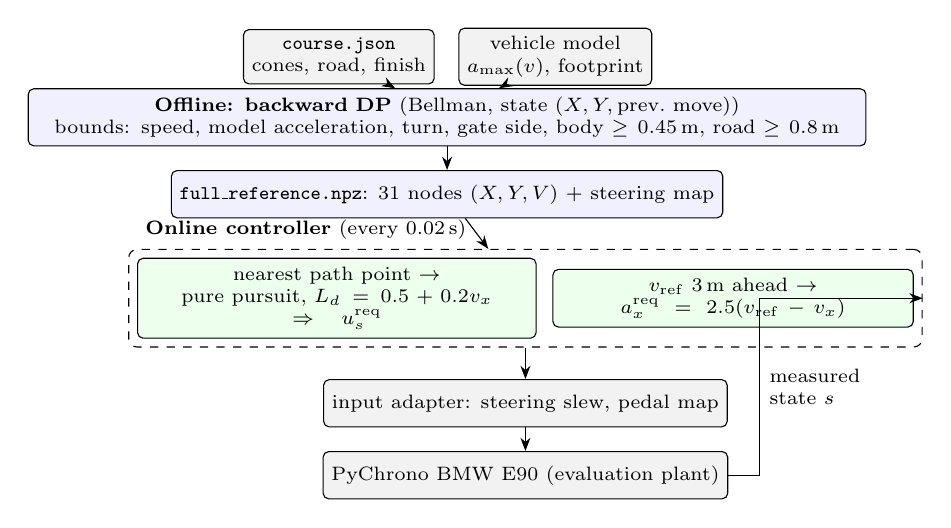
\begin{tikzpicture}[font=\scriptsize, >=Stealth,
  box/.style={draw, rounded corners=2pt, align=center, inner sep=3pt, minimum height=6mm},
  off/.style={box, fill=blue!6}, on/.style={box, fill=green!7}, fix/.style={box, fill=gray!10}]
\node[fix] (course) {\texttt{course.json}\\cones, road, finish};
\node[fix, right=3mm of course] (model) {vehicle model\\$a_{\max}(v)$, footprint};
\node[off, below=4mm of $(course)!0.5!(model)$, text width=0.86\columnwidth] (dp)
 {\textbf{Offline: backward DP} (Bellman, state $(X,Y,\text{prev.\ move})$)\\
  bounds: speed, model acceleration, turn, gate side, body $\ge0.45$\,m, road $\ge0.8$\,m};
\node[off, below=3mm of dp] (ref) {\texttt{full\_reference.npz}: 31 nodes $(X,Y,V)$ + steering map};
\node[on, below=5mm of ref, xshift=-14mm, text width=0.40\columnwidth] (pp)
 {nearest path point $\rightarrow$\\ pure pursuit, $L_d=0.5+0.2v_x$\\ $\Rightarrow u_s^{\rm req}$};
\node[on, right=2mm of pp, text width=0.36\columnwidth] (sp)
 {$v_{\rm ref}$ 3\,m ahead $\rightarrow$\\ $a_x^{\rm req}=2.5(v_{\rm ref}-v_x)$};
\node[draw, dashed, rounded corners=3pt, fit=(pp)(sp), inner sep=3pt,
 label={[font=\scriptsize]above left:{\textbf{Online controller} (every 0.02\,s)}}] (ctrl) {};
\node[fix, below=4mm of ctrl] (adapt) {input adapter: steering slew, pedal map};
\node[fix, below=3mm of adapt] (plant) {PyChrono BMW E90 (evaluation plant)};
\draw[->] (course) -- (dp); \draw[->] (model) -- (dp);
\draw[->] (dp) -- (ref); \draw[->] (ref) -- (ctrl);
\draw[->] (ctrl) -- (adapt); \draw[->] (adapt) -- (plant);
\draw[->] (plant.east) -- ++(4mm,0) |- node[pos=0.25, right, align=left]{measured\\ state $s$} (ctrl.east);
\end{tikzpicture}
\caption{My Full-mode method: an offline backward-DP planner turns the course
and model-based bounds into a minimum-time REF reference; a feedback tracker
converts it into steering and acceleration requests every 0.02\,s. Easy mode
uses the same DP on the published lattice, with the professor's tracker.}
\label{fig:method}
\end{figure}

% =====================================================================
\section{Own Validation}
% =====================================================================
\subsection{Setup and reproducibility}
All runs use the supplied runner, course and Conda environment (Windows,
Python 3.12.14, PyChrono 10.0.0, headless). The same plans and controllers were
also replayed on an independent Linux installation of PyChrono 10.0.0; results
agreed to about 1\,ms and 0.5\,mm (e.g.\ 24.0460/24.0455\,s and
0.7383/0.7378\,m), so the reported numbers are reproducible and a small
clearance buffer covers platform differences.

\subsection{Results and baselines}
Table~\ref{tab:results} compares my solutions with the supplied baselines. My
Full controller is \textbf{2.0$\times$ faster than the example controller},
1.35\,s faster than my Easy plan, and only 0.9\,s above the physical floor of
about 14.1\,s that I computed for a \emph{straight, cone-free} 145\,m run with
the model's maximum acceleration and an 11.5\,m/s cap. Fig.~\ref{fig:traj}
shows the paths: Full v2 passes the cones every $\approx1.41$\,s
($\approx10.6$\,m/s) at $|Y_{\rm REF}|=1.72$--$2.04$\,m and crosses the line at
11.53\,m/s (Fig.~\ref{fig:speed}).

\begin{table}[t]
\centering
\caption{PyChrono results (basic course, all 8 gates passed)}
\label{tab:results}
\footnotesize
\setlength{\tabcolsep}{3pt}
\begin{tabular}{@{}lccc@{}}
\toprule
Solution & time (s) & clearance (m) & survives shift \\
\midrule
Example controller (Full) & 30.660 & 0.881 & -- \\
Example plan, 73 st.\ (Easy) & 36.548 & 0.485 & -- \\
Professor's DP, 2.5\,m (Easy) & 24.074 & 0.734 & -- \\
My DP, 2.5\,m, 48 st.\ (Easy) & 24.046 & 0.738 & 0.6\,m \\
My tuned DP, 32 st.\ (Easy) & 16.333 & 0.440 & 0.4\,m \\
My DP + tracker v1 (Full) & 15.324 & 0.525 & 0.5\,m \\
\textbf{My DP + tracker v2 (Full)} & \textbf{14.985} & \textbf{0.377} & \textbf{0.35\,m} \\
\bottomrule
\end{tabular}
\end{table}

\begin{figure*}[t]
\centering
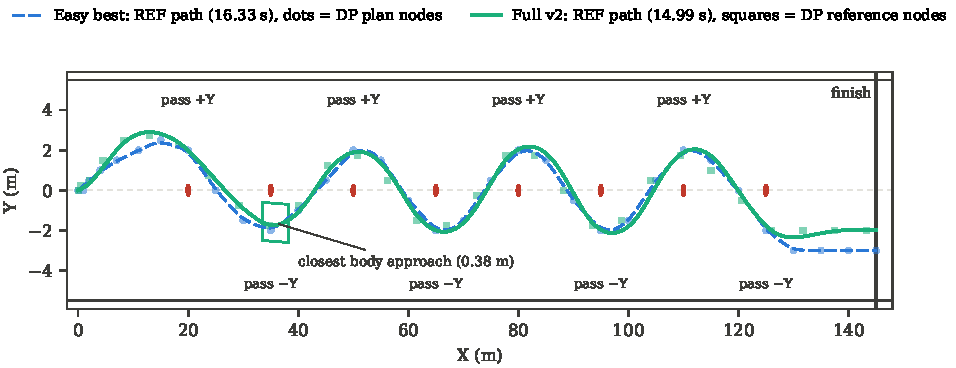
\includegraphics[width=\textwidth]{figures/fig_trajectories.pdf}
\caption{Top view of the measured REF paths (lateral scale exaggerated about
3$\times$). Dots: Easy DP plan nodes; squares: Full DP reference nodes. The
footprint drawn at cone~1 marks the closest body approach of Full v2 (0.38\,m),
which happens just after REF has passed the cone, when the rear of the turning
car swings toward it. Both solutions stay on the side of the road after the
last cone instead of returning to the centre line.}
\label{fig:traj}
\end{figure*}

\begin{figure}[t]
\centering
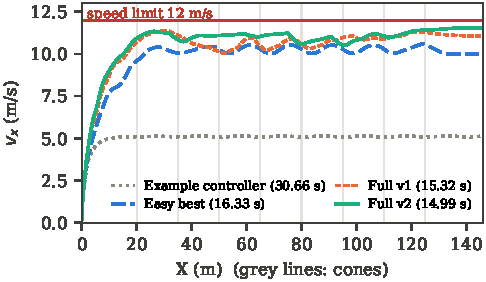
\includegraphics[width=\columnwidth]{figures/fig_speed.pdf}
\caption{Measured forward speed. Full mode accelerates harder at the start
(model-based acceleration bound) and runs at 10.6--11.5\,m/s instead of the
10\,m/s cap of the Easy lattice.}
\label{fig:speed}
\end{figure}

\subsection{Tuning evidence and the choice of each value}
Every bound and gain was chosen by an outer loop: plan, drive in PyChrono, and
compare finish time with minimum clearance (Fig.~\ref{fig:tradeoff},
Tables~\ref{tab:easy}--\ref{tab:full} in the Appendix). My selection rule was
the fastest success with clearance $\ge0.3$\,m (about 600$\times$ the measured
platform difference and $\approx2\times$ the largest lateral prediction RMSE in
\texttt{MODEL.md}). The selected Easy plan is the fastest successful Easy run
overall, so the choice holds for any buffer up to 0.44\,m. For the Full-mode
tracker gains I added a stability condition: the neighbouring lookahead settings
must also keep $\ge0.3$\,m. Two settings are 0.05--0.06\,s faster with
$\ge0.3$\,m (Table~\ref{tab:full}), but each has a neighbour at only
0.19--0.20\,m; $0.5+0.2v_x$ is the fastest setting whose neighbours both pass.

Main findings: (1)~Relaxing the suggested turning bounds made the Easy plan
faster \emph{and} safer (19.66\,s/0.33\,m $\rightarrow$ 16.33\,s/0.44\,m),
because the car reaches the side quickly instead of drifting near the cone.
(2)~Every 31-stage Easy plan crashed, although each was feasible on paper: the
fixed tracker cuts corners (planned 2.0\,m, measured 1.85--1.90\,m at the
gates), so 32 stages is the practical floor. (3)~In Full mode, a 5.5\,m
lookahead cut the corner and hit cone~2; shorter lookahead gives more
clearance. (4)~After the planner was made faster (v1 $\rightarrow$ v2,
$\approx10.3\rightarrow10.6$\,m/s through the cones), the short v1 lookahead
($0.5+0.1v_x$) became \emph{unstable}: the steering oscillation grew until the
steering saturated at $\pm0.8$ and the car left the road after cone~6. A larger
road margin did not help, which shows that the cause was the tracker, not the
path. This is why I chose the lookahead with a margin to the unstable and the
corner-cutting side instead of the fastest single run.

\begin{figure}[t]
\centering
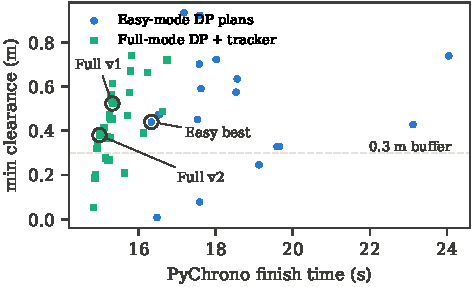
\includegraphics[width=\columnwidth]{figures/fig_tradeoff.pdf}
\caption{Finish time vs.\ minimum clearance of all successful tuning runs
(failures are listed in the Appendix). Circled: the selected solutions.}
\label{fig:tradeoff}
\end{figure}

\subsection{Robustness and model checks}
To test whether \texttt{min\_clearance\_m} is a real safety margin, I kept each
solution fixed and moved every cone toward the car by $s$ (local course copies
with \texttt{cone\_centers\_m}). Clearance falls about one-to-one with $s$, and
each solution fails close to its measured clearance (Fig.~\ref{fig:robust}). The
finish time is unchanged, which also shows that my controllers do not use the
cone positions online. Replaying the recorded v2 requests (replicated run) with
\texttt{validate\_requests.py} gave REF lateral RMSE of 0.024/0.078/0.273\,m and
speed RMSE of 0.097/0.157/0.282\,m/s at 0.5/1/2\,s horizons: the supplied model
is accurate for short horizons with feedback, but not for 2\,s open-loop use.

\begin{figure}[t]
\centering
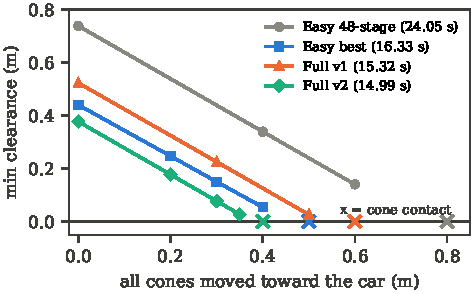
\includegraphics[width=\columnwidth]{figures/fig_robustness.pdf}
\caption{Robustness test: the same solution driven on harder courses with all
cones shifted toward its path. The clearance drops one-to-one and contact occurs
near the measured clearance. (Full v1 values from the replicated runs; the
others from my PC.)}
\label{fig:robust}
\end{figure}

\subsection{Limitations}
(i)~The controller tracks a precomputed reference and does not use cone
positions online, so a new course requires re-planning. (ii)~Tracker stability
depends on the reference speed (lookahead and speed must be tuned together).
(iii)~The DP uses approximations: chord headings for the body check, a virtual
lateral acceleration over 0.5\,s stages (bound 8, measured peaks
8.8--9.2\,m/s$^2$), and an optimistic first stage from rest. (iv)~The speed loop
gains (2.5, 3\,m preview) were not tuned. (v)~Tests are deterministic and limited
to the basic course and cone-shift variants. (vi)~Without Numba,
\texttt{dynamics.predict} costs about 0.3\,ms per call, so an online rollout with
several candidates and a 1\,s horizon did not fit into the 20\,ms control period.

% =====================================================================
\section{Conclusion}
% =====================================================================
A single backward-DP formulation, extended with model-based acceleration bounds
and exact footprint and road checks, solved both modes: 16.333\,s in Easy mode
and \textbf{14.985\,s in Full mode} with 0.377\,m minimum clearance, against
30.660\,s for the example controller. The key lessons were that a plan that is
feasible on paper must be validated on the plant, and that the tracking
controller limits how aggressive the plan can be. The main limitation is that the
controller does not react to cones online; the natural next step is a rollout
(one-step lookahead with this controller as base policy) using a vectorized copy
of the vehicle model and the real cone positions.

\noindent\textbf{AI use:} I used Claude (Anthropic) through the Claude app
(configured model: claude-opus-5-5) as a tutor and coding assistant: explaining
the repository and course concepts step by step, drafting and debugging code
(\texttt{easy\_dp.py}, \texttt{full\_dp.py}, the controller and the test
scripts), replicating runs on a separate Linux installation, proposing tuning
sweeps, making the figures, and drafting this report. I directed the work (Easy
first, then Full; keeping benchmarks; adding the robustness test; asking for
further optimization; choosing the final speed--safety trade-off), ran all code
on my own PC, reproduced the reported results, and checked the explanations; for
example, I questioned an early tire-grip argument, which led to the corrected
trackability explanation above. \todo{adjust to your exact usage}

% =====================================================================
\appendix
% =====================================================================
\subsection{Easy-mode tuning (PyChrono)}
\begin{table}[h]
\centering
\caption{Easy DP plans (other bounds = suggested values)}
\label{tab:easy}
\footnotesize
\setlength{\tabcolsep}{2.5pt}
\begin{tabular}{@{}cccccc@{}}
\toprule
gate (m) & $|\Delta\chi|$ & $a_{\rm lat}$ & stages & time (s) & clear.\ (m)\\
\midrule
1.0 & 0.31 & 6 & 31 & contact & $-0.002$\\
1.5 & 0.31 & 6 & 32 & 16.477 & 0.008\\
1.75 & 0.31 & 6 & 37 & 19.121 & 0.246\\
2.0 & 0.31 & 6 & 38 & 19.655 & 0.328\\
2.25 & 0.31 & 6 & 46 & 23.121 & 0.428\\
2.5 & 0.31 & 6 & 48 & 24.046 & 0.738\\
2.0 & 0.40 & 7 & 34 & 17.53 & 0.45\\
2.0 & 0.40 & 8 & 32 & 16.54 & 0.47\\
\textbf{2.0} & \textbf{0.50} & \textbf{8} & \textbf{32} & \textbf{16.333} & \textbf{0.440}\\
2.0 & 0.60 & 8 & 32 & 16.33 & 0.44\\
1.75 & 0.50 & 8 & 32 & 16.51 & 0.47\\
2.25 & 0.50 & 8 / 9 & 35 / 34 & 18.02 / 17.58 & 0.72 / 0.70\\
2.5 & 0.50 & 8 / 10 & 36 / 34 & 18.53 / 17.59 & 0.57 / 0.92\\
2.5 & 0.50 & none & 33 & 17.18 & 0.93\\
2.5 & 0.60 & none & 32 & contact & --\\
2.0 & 0.50 & 10 / none & 31 & contact & --\\
1.75 & 0.50 & 9 & 31 & contact & --\\
\bottomrule
\end{tabular}
\end{table}
Other Easy tests: road strip 3.5/4.0\,m changed nothing; a footprint margin
instead of a gate margin (gate 1.2\,m) gave 17.585\,s/0.078\,m (0.3),
19.126\,s/0.246\,m (0.5) and 19.657\,s/0.328\,m (0.7). With a 4\,m/s$^2$ bound,
31 stages is the arithmetic minimum ($1+2+3+4$\,m, then $27\times5$\,m).
Robustness of the 48-stage plan: 0.738/0.339/0.140\,m for shifts 0/0.4/0.6\,m,
contact at 0.8\,m. The professor's narrow 0.5\,m example plan touched cone~0
($-0.002$\,m) although it passed on the correct side, which motivated all
margins.

\subsection{Full-mode tuning (PyChrono)}
\begin{table}[h]
\centering
\caption{Full mode: body margin, $a_{\rm lat}$ and lookahead $L_d=b+g\,v_x$}
\label{tab:full}
\footnotesize
\setlength{\tabcolsep}{2.5pt}
\begin{tabular}{@{}lcccc@{}}
\toprule
lattice, body, $a_{\rm lat}$ & $b/g$ & time (s) & clear.\ (m) & note\\
\midrule
v1, 0.45, 8 & 2.0/0.35 & contact & -- & cone 2\\
v1, 0.45, 8 & 1.0/0.2 & 15.215 & 0.267 & \\
v1, 0.45, 8 & 0.5/0.2 & 15.250 & 0.367 & \\
v1, 0.45, 8 & 1.0/0.1 & 15.283 & 0.452 & \\
\textbf{v1, 0.45, 8} & \textbf{0.5/0.1} & \textbf{15.324} & \textbf{0.525} & \textbf{v1}\\
v1, 0.45, 9.5 & 4 settings & 15.23--15.37 & 0.27--0.52 & all ok\\
v1, 0.6, 8 & 5 settings & 15.63--15.82 & 0.21--0.74 & all ok\\
v1, 0.6, 9.5 & 3 of 4 & -- & -- & fail\\
v1, 0.8 / 1.0, 8 & 1.0/0.2 & 16.24 / 16.74 & 0.66 / 0.72 & \\
v2, 0.45, 8 & 0.5/0.1 & road dep. & -- & unstable\\
v2, 0.45, 8 & 0.5/0.15 & 15.101 & 0.414 & \\
\textbf{v2, 0.45, 8} & \textbf{0.5/0.2} & \textbf{14.985} & \textbf{0.377} & \textbf{final}\\
v2, 0.45, 8 & 0.5/0.25 & 14.929 & 0.320 & \\
v2, 0.45, 8 & 0.5/0.3 & 14.877 & 0.187 & \\
v2, 0.45, 8 & 1.0/0.15 & 14.994 & 0.385 & \\
v2, 0.45, 8 & 1.0/0.2--0.3 & 14.83--14.93 & 0.05--0.33 & \\
v2, 0.55, 8 & 8 settings & 15.14--15.33 & 0.28--0.61 & all ok\\
\bottomrule
\end{tabular}
\end{table}
v1 lattice: $h_X=0.5$\,m, $m\le11$ (1\,m/s speed steps; 15.0\,s planned);
v2: $h_X=0.25$\,m, $m\le23$, fractional finish cost, road check (14.65\,s
planned). Development issues: an acceleration bound evaluated at the start speed
($a_{\max}(0)\approx1.98$\,m/s$^2$) and a 90\,\% scale made the start from rest
infeasible (1\,m/s needs 0.459\,s), which led to the integral time bound; a
$\Delta=0.25$\,s lattice was also infeasible from rest. Full v1 robustness:
0.225/0.026\,m at shifts 0.3/0.5\,m, contact at 0.6\,m.

\subsection{Setup issues and reproduction}
Setup: \texttt{conda} was not on the PowerShell path (fixed with
\texttt{conda init powershell} and the execution policy), and Windows Smart App
Control intermittently blocked NumPy and PyChrono DLLs (not a code problem).
Reproduction: \texttt{python easy\_dp.py --gate-margin 2.0 --max-angle-change 0.5
--max-lat-accel 8 --output easy\_plan.json}; \texttt{python full\_dp.py}
(defaults are the final settings) writes \texttt{full\_reference.npz}, which
\texttt{controller.py} loads from its own folder. Only NumPy is needed. Tools:
\texttt{robustness\_test.py}, \texttt{clearance\_by\_cone.py},
\texttt{make\_figures.py}.

\end{document}
